\chapter{Packages}

\section{Client}

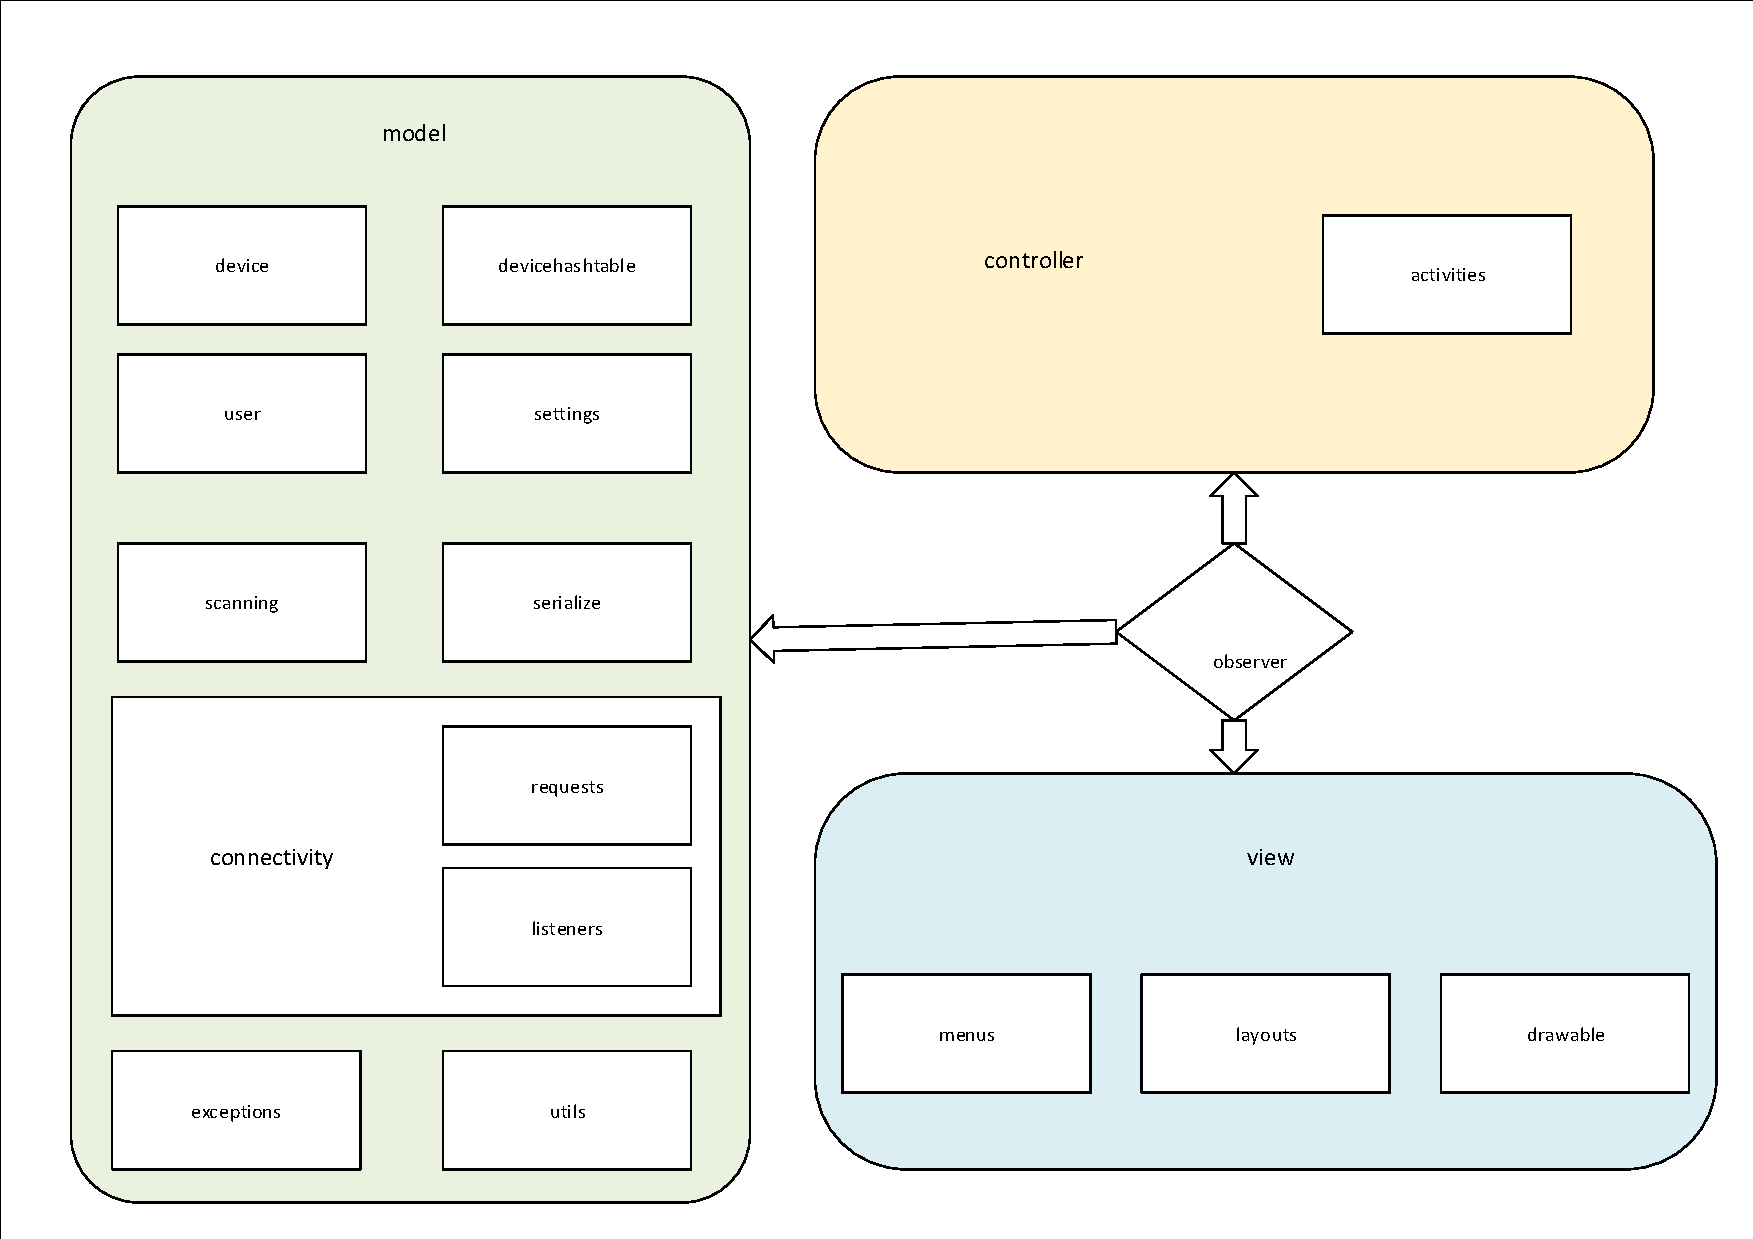
\includegraphics[width=\textwidth]{img/client_packages}

\subsection{model}
The client model contains data persistence and business logic. How data is acquired or assembled should be transparent for view controller. This is why connectivity is handled inside the model.
\subsubsection{model.user}
This package contains data regarding user authentication.
\subsubsection{model.device}
The device package manages data about scanned BT-Devices and their locations.
\subsubsection{model.serialize}
This package provides classes that can serialize data before it is sent to the server.
\subsubsection{model.connectivity}
This package provides classes that manage the communication with the server. It defines all request types and listeners to handle them.
\subsubsection{model.devicehashtable}
This package contains the table of devices that are currently being tracked.
\subsubsection{model.scanning}
This package provides the functionality to perform bluetooth scans in the background.
\subsubsection{model.utils}
This package contains various utility classes.
\subsection{controller}
The client controller is responsible for displaying the appropriate views and routing user input into the model.
\subsubsection{controller.activities}
Android activity classes for each possible screen.
\subsubsection{controller.fragments}
Android fragments for pop-up dialogs.
\subsection{view}
The view contains all presentation templates. 
\subsubsection{view.menus}
Views for menu items, such as the options menu.
\subsubsection{view.layouts}
Layout templates for all possible screens. 
\subsubsection{view.drawable}
Any additional presentation resources.



\section{Server}
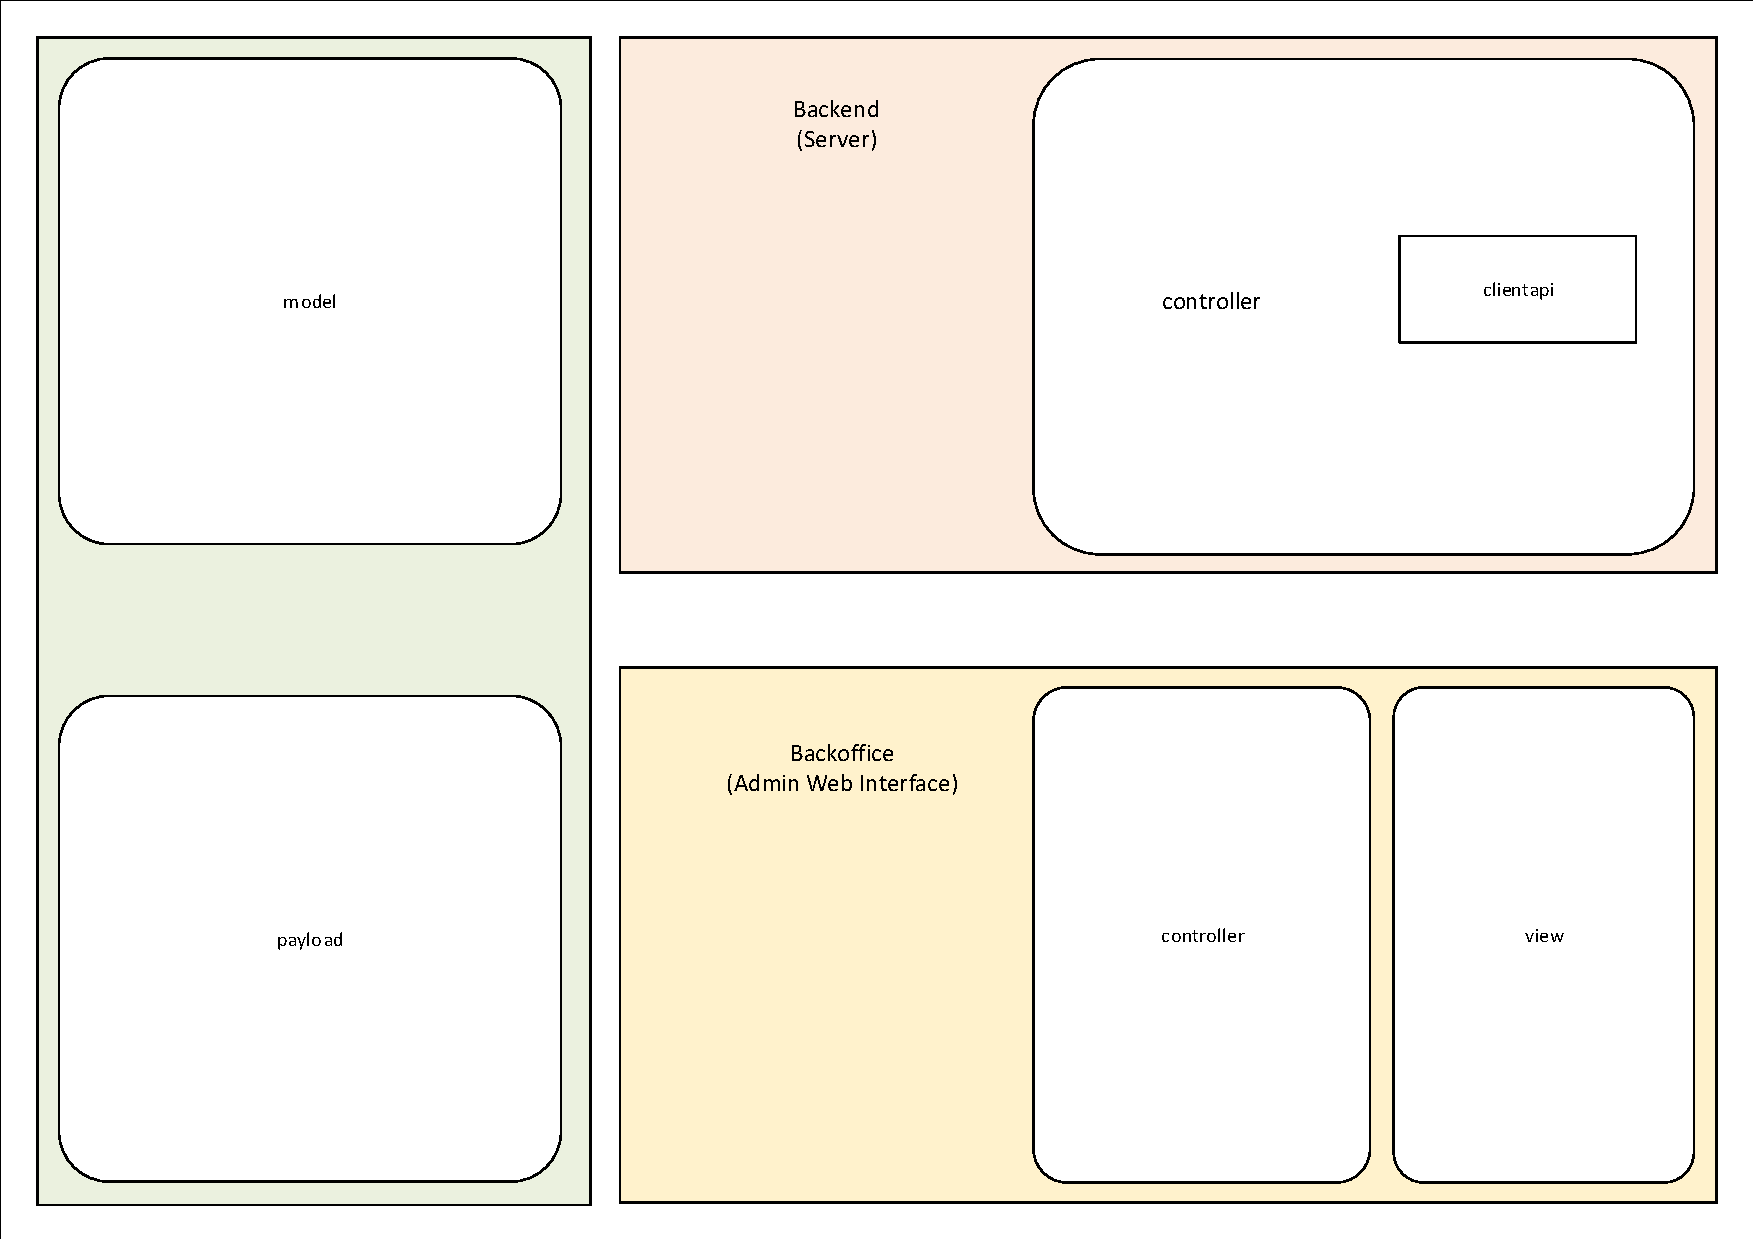
\includegraphics[width=\textwidth]{img/server_packages}

\subsection{model}
The server model contains data persistence and business logic. The same model can be used for backend and backoffice processes.
\subsection{backend}
The backend is the process that handles communication with the clients and user authentication. It updates and relays the table of devices that are currently being tracked. It also relays location data to the owner.
\subsubsection{backend.controller}
The controller is responsible for receiving requests and updating the model.
\subsubsection{backend.controller.api}
The client api provides an interface for the communication with the client.
\subsection{backoffice}
The backoffice is a web interface that allows server administration and data manipulation for authorized Administrators.
\subsubsection{backoffice.controller}
The backoffice controller is responsible for displaying the appropriate templates and routing user input into the model.
\subsubsection{backoffice.view}
The view consists of website templates and style resources.
\section{Shared Packages}
\subsection{payload}
The payload classes represent the various types of data that can be transferred between client and server.